\chapter{Introdução}

O desenvolvimento de software passou, e de certa forma ainda passa, por uma fase
conhecida como \emph{crise do software}, termo utilizado pela primeira vez por
\citeonline{HumbleProgrammer}. A Engenharia de Software surgiu
\cite{NaurRandell} numa tentativa de contornar esta crise. No entanto, a
Engenharia de Software foi baseada em algumas considerações equivocadas:

\begin{itemize}
    \item
        O desenvolvimento de software é um trabalho executado por trabalhadores
        manuais e não um trabalhadores do conhecimento \cite[38]{XPTeles}.
    \item
        Ao tentar com bastante afinco, consegue-se antecipar todo o conjunto de
        requisitos e reduzir os custos eliminando as mudanças
        \cite{TheBusinessOfInnovation}.
\end{itemize}

Isso fez com que a Engenharia de Software falhasse na sua tentativa de contornar
tal crise, pois com o passar dos anos, o mercado demanda e espera software
inovadores e de alta qualidade, que sejam adequados a suas necessidades - e o
mais rápido possível \cite{TheBusinessOfInnovation}.

O desenvolvimento ágil de software, que neste ano de 2011 completa 10 anos,
surgiu \cite{AgileManifesto} para resolver esta crise que a Engenharia de
Software tradicional não conseguiu, focando nas pessoas ao invés do processo e
abraçando as mudanças ao invés de evitá-las. De acordo com
\citeonline{PMNetworkFailureDrop}, o \textit{Chaos Manifesto 2011}\footnote{O
\textit{Chaos Manifesto} é uma pesquisa bienal realizada pelo \textit{The
Standish Group} e teve início em 1994. As pesquisas publicadas em um ano
representam os dados do ano anterior.} mostra que os resultados de 2010
representam, desde sua primeira edição, a maior taxa de sucesso nos projetos de
desenvolvimento de software, que aumentou de 32\% em 2008 para 37\% em 2010.
Segundo \citeonline{ResumoChaosReport}, o \textit{The Standish Group} conclui
que uma das principais razões para o aumento da taxa de sucesso foi a utilização
das metodologias ágeis, que cresce a uma taxa de 22\%
CAGR\footnote{\href{http://en.wikipedia.org/wiki/Compound_annual_growth_rate}
{Compound annual growth rate}} e hoje são adotados em 9\% de todos os projetos
de TI em andamento e em 29\% dos novos projetos.

Como o desenvolvimento ágil é relativamente novo, diversos métodos e técnicas
vem sendo desenvolvidos tendo como base os princípios e valores ágeis
\cite{BDDRodrigo}. Sendo técnicas emergentes, ainda são pouco discutidas no meio
acadêmico, este trabalho pretende contribuir com esta discussão e, de certa
forma, com a introdução de técnicas vindas do mercado na academia.



\section{Objetivos}

O objetivo principal do presente trabalho é contribuir com a introdução de
técnicas e discussões surgidas no mercado para a academia, além de compilar
informações, hoje dispersas, sobre as vantagens e desvantagens da utilização de
tais técnicas.

Existem também algumas questões em aberto no desenvolvimento ágil de software,
que serão alvo de discussão neste trabalho.

\section{Metodologia}

Será feita uma explanação sobre cada técnica e uma discussão mostrando onde são
melhor aplicadas, comparando as diferentes abordagens para cada técnica, bem
como as vantagens e desvantagens em seu uso.

Como base para a discussão, será utilizado o
kaban-roots\footnote{\href{http://github.com/hugomaiavieira/kanban-roots}
{http://github.com/hugomaiavieira/kanban-roots}}, que está sendo desenvolvido em
conjunto com o presente trabalho.

O kanban-roots é um kanban\footnote{Nesse contexto, kanban é um quadro para
visualização do fluxo de trabalho (tarefas) em um projeto.} online para auxiliar
a organização de tarefas de um projeto. O kanban-roots já está em produção
e vem sendo utilizado com sucesso por algumas empresas.

\begin{figure}[h]
    \center
    \caption{Tela do  kanban-roots}
    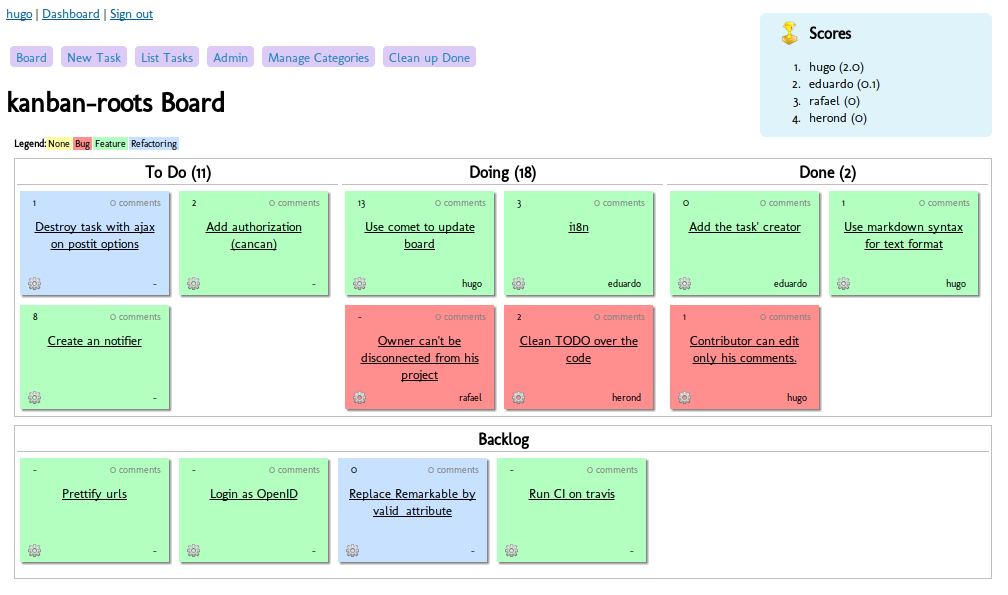
\includegraphics[scale=0.45]{images/kanban-roots}
    \label{tela_kaban_roots}
\end{figure}
